\documentclass[12pt]{article}
\usepackage[margin=0.5in]{geometry} 
\usepackage{amsmath,amsthm,amssymb,amsfonts, enumitem, fancyhdr, color, comment, graphicx, environ}
\usepackage{course}
\usepackage{cse468-Spring24}
\usepackage{program}
\usepackage{fancybox}
\usepackage{adjustbox}
\usepackage{quantikz}
\usepackage{../bbkey}
\def\SquareOutline{%
\path (0,0) rectangle (1,1);%
}%
\def\Gate#1{\mbox{\textbf{#1}}}
\def\X{\Gate{X}}
\def\Y{\Gate{Y}}
\def\Z{\Gate{Z}}
\def\I{\Gate{I}}
\def\H{\Gate{H}}
\def\QZero{\ket{0}}
\def\QState#1{\ensuremath{\psi_{#1}}}

\def\Obox#1{\Ovalbox{\hbox to 1ex{\vrule width 0pt height 1ex\hss #1\hss}}}
\def\TFMarked#1#2{\ \stackbox[l][m]{\Obox{#1}~\textbf{true}\\\Obox{#2}~\textbf{false}}}
\def\TF{\TFMarked{\relax}{\relax}}
\def\TFH{\Obox{\relax}~\textbf{true}~~~\Obox{\relax}~\textbf{false}}
\def\exp#1{\ensuremath{e^{#1}}}
\newcommand{\Blank}[1][1in]{\mbox{\vrule width #1 depth 2pt}\vrule width 0pt height 2.0em}
\def\BlQb{\mbox{\ensuremath{\Blank[4em]\ket{0}+\Blank[4em]\ket{1}}}}
\newcommand{\Blanket}[1][3em]{%
\mbox{\ensuremath{|\,\Blank[#1]\,\rangle}}}

\def\Tall{\vrule width 0pt height 2em depth 0.5em}

\def\SQB#1#2{%
\ensuremath{%
\begin{pmatrix*}[r] #1 \\ #2\end{pmatrix*}}}

\def\SQBB{\SQB{\Blank[2em]}{\Blank[2em]}}

\def\DQB#1#2#3#4{%
\ensuremath{%
\begin{pmatrix*}[r] #1 \\ #2 \\ #3 \\ #4\end{pmatrix*}}}
\def\DQBB{\DQB{\Blank[2em]}{\Blank[2em]}{\Blank[2em]}{\Blank[2em]}}

\def\FactorProof{%
\begin{align*}
\SQB{a}{b} \otimes \SQB{c}{d} &= \DQBB{} \mbox{ (copy this from your \QState{2} answer top of page)}\\
a\cdot c &= \Blank[3em] \\
a\cdot d &= \Blank[3em] \\
b\cdot c &= \Blank[3em] \\
b\cdot d &= \Blank[3em]
\end{align*}
What is the contradiction, if any?
\LeaveSpace{2in}
}

\begin{document}

\begin{assignment}{Exam I}{6 March 2024}{In GradesScope by 22 March 2024, 9 AM CDT}

{\small {\large \fbox{READ THIS before starting!}}
This exam is open-book, open-notes, open-Internet, but you must do this
work on your own without contact or conversations with any person.
Because this exam is given in a distributed manner, no questions will be answered, and no clarifications will be given.  State your assumptions and count on us to be fair and flexible, especially if we have been unclear.


Your work must be legible.  Work that is
difficult to read will receive no credit.  There is a blank page at the end
if you want to show extra work there.  To assure no problems with GradeScope,
you should
print out this exam, complete it on paper, and scan it in with a full-page
scanner.  You can be more creative but if you do not properly register the
pages with GradeScope, credit will not be given.

There are ??? points available for this exam, but it will only be scored out of 100.  Extra points earned here will count toward your total exam grade, including Exam~II.

You must sign the pledge below for your exam to count.  Any cheating will
cause the students involved to receive an F for this course. Other unpleasant
actions
may be taken.

You must fill in your identifying information correctly.  You must upload this
completed exam to GradeScope properly by the due date and time.
}

\begin{center}\large
\begin{tabular}{|c|c|c|} \hline
\multicolumn{3}{|c|}{{\bf Print  clearly} the following information:}  \\ \hline
\multicolumn{3}{|l|}{Name (print clearly):\Tall{}\hbox to 3in{\hss}}  \\ \hline
\multicolumn{3}{|l|}{Student 6-digit ID (print {\it really} clearly):\Tall{}\hbox to 3in{\hss}} \\ \hline
\end{tabular}
\end{center}

{\bf Pledge:} On my honor, I have neither
given nor received any unauthorized aid on this exam.

Signed:  \Blank\Blank\Blank\Blank \\ \hbox to 5em{\hss}(Be 
sure you filled in your information in the box above!)
%
%
%
\clearpage
\begin{enumerate}
\item\Points{20+4} For the \textbf{true}/\textbf{false} questions below, indicate your response by marking an~\textbf{x} in the appropriate box, like this:
\TFMarked{\textbf{x}}{\relax} or \TFMarked{\relax}{\textbf{x}}.  Each is worth 2 points, so there are 4 points of extra credit here. \textbf{Remember that $\equiv$ means equal up to a global phase.}


\begin{itemize}
    \item When an unpolarized photon hits a polarizing filter, that constitutes a measurement of a photon's polarization.~\TF{}
    \item Each of the Pauli matrices (\X, \Y, and \Z) is its own inverse.~\TF{}
    \item The states $\ket{+}=\frac{1}{\sqrt{2}}\SQB{1}{1}$ and $\ket{-}=\frac{1}{\sqrt{2}}\SQB{1}{-1}$ differ only by a global phase.~\TF{}
    \item The states $i\SQB{0}{1}$ and $\SQB{0}{-1}$ differ only by a global phase.~\TF{}
    \item The conjugate transpose of \SQB{1}{i} is $\left(-1\ \  -i\right)$.~\TF{}
    \item For \emph{all} values of $\theta$, $|e^{i\,\theta}|=1$.\TF{}
    \item For the Pauli matrices, $\Gate{X}\Gate{Y}\Gate{Z}\Gate{Z}\Gate{Y}\equiv\Gate{X}$~\TF{}
    \item The state \[\frac{\ket{10}+\ket{11}}{\sqrt{2}}\] is an entangled state.~\TF{}
    \item The state obtained after measuring the left qubit of \[\frac{\ket{00}+\ket{11}}{\sqrt{2}}\] is an entangled state.~\TF{}
    \item The state \[\Gate{CNOT}\left(\frac{\ket{00}+\ket{11}}{\sqrt{2}}\right)\] is an entangled state.~\TF{}
    \item For all states $\ket{\psi}$, $\Gate{X}\Gate{Z}\ket{\psi}\equiv\Gate{Z}\Gate{X}\ket{\psi}$~\TF{}
       \item Following the measurement of a single qubit in the standard basis, the number of possible states of that qubit is uncountably infinite.~\TF{}

\end{itemize}

\long\def\GenTable#1#2{%
\GenTableDiff{#1}{#2}{#1}{#2}}%
\long\def\GenTableDiff#1#2#3#4{%
\begin{center}
\begin{tabular}{ccc}
Alice & Bob & Possible Outcome? \\
\ensuremath{#1}    & \ensuremath{#3}  & \TFH \\[0.5em]
\ensuremath{#1}    & \ensuremath{#4}  & \TFH \\[0.5em]
\ensuremath{#2}    & \ensuremath{#3}  & \TFH \\[0.5em]
\ensuremath{#2}    & \ensuremath{#4}  & \TFH
\end{tabular}
\end{center}
}
\def\EmptyFour{%
\frac{1}{\Blank[2em]} \begin{pmatrix*}[r]
      \Blank[1.5em] \\
      \Blank[1.5em] \\
      \Blank[1.5em] \\
      \Blank[1.5em]
    \end{pmatrix*}
}
\def\EmptyFourByFour{%
\frac{1}{\Blank[2em]} \begin{pmatrix*}[r]
 \Blank[3em]{} & \Blank[3em]{} & \Blank[3em]{} & \Blank[3em]{} \\
 \Blank[3em]{} & \Blank[3em]{} & \Blank[3em]{} & \Blank[3em]{} \\
 \Blank[3em]{} & \Blank[3em]{} & \Blank[3em]{} & \Blank[3em]{} \\
 \Blank[3em]{} & \Blank[3em]{} & \Blank[3em]{} & \Blank[3em]{}\end{pmatrix*}}
\def\Bell{%
\BellTwo{00}{11}}
\def\BellTwo#1#2{%
\ensuremath{\frac{\ket{#1}+\ket{#2}}{\sqrt{2}}}}

\clearpage\item\label{prob:follow}\Points{20} Alice and Bob prepare to participate in one of the
many schemes we've studied this semester in which they begin with the 
Bell (also called an EPR) state:
\[ \ket{\psi_{1}} = \frac{\ket{00}+\ket{11}}{\sqrt{2}} = \frac{1}{\sqrt{2}} \begin{pmatrix} 1\\0\\0\\1\end{pmatrix}\]
When they separate, Alice takes the left qubit and Bob takes the right qubit.
They each then measure their qubit in a basis as described below.

\begin{enumerate}
\item Suppose they each measure $\ket{\psi_{1}}$ in the computational (\textbf{Z})
basis.
Which measurement outcomes are possible for this state?
\GenTable{0}{1}

\item
In class it was shown that
\[
\ket{\psi_{1}} = \Bell{} = \frac{\ket{++}+\ket{--}}{\sqrt{2}}
\]
by showing the associated column vectors are mathematically equal:
\[
\ket{\psi_{1}} = \frac{1}{\sqrt{2}} \begin{pmatrix} 1\\0\\0\\1\end{pmatrix}
= \frac{1}{\sqrt{2}} \left[ \frac{1}{2}\begin{pmatrix}1\\1\\1\\1\end{pmatrix}
+  \frac{1}{2}\begin{pmatrix*}[r]1 \\-1\\-1\\1\end{pmatrix*}\right]
\]
After separation, they each measure their qubit of $\ket{\psi_{1}}$ in the
\textbf{X} basis, each using a magical \textbf{X}-basis measuring device.  

Which measurement outcomes are possible?
\GenTable{+}{-}
\Continued{}

\item This time, due to miscommunication, Alice measures her qubit in the \textbf{X} basis
but Bob measures his in the computational basis.  
This is achieved by applying the unitary gate $\textbf{H}\otimes\textbf{I}$
to the state $\ket{\psi_{1}}=\frac{1}{\sqrt{2}}\begin{pmatrix}1\\0\\0\\1\end{pmatrix}$.
In other words, Alice applies \textbf{H} to her qubit while Bob does nothing
to his.
\[ \textbf{H}\otimes\textbf{I} = \EmptyFourByFour{} \]
The state resulting from that operation is:

\[ \ket{\psi_{2}} = \left(\textbf{H}\otimes\textbf{I}\right)\ket{\psi_{1}} = \EmptyFour{} \]

Alice and Bob each measure their qubit of $\ket{\psi_{2}}$ in the computational
basis.  Which of the following measurement outcomes are possible?
\GenTable{0}{1}
Finally, they repply
$\textbf{H}\otimes\textbf{I}$ to the measured outcome.

In which of the following states could the quantum system be now?
\GenTableDiff{+}{-}{0}{1}
\end{enumerate}

\clearpage\item\Points{20}
We next explore the strength of commitment Alice and Bob bring to their
entanglement, as Eve enters the picture and seeks to become just as entangled
with Alice and Bob as they are with each other.

Alice and Bob share the left and right qubits respectively of $\ket{\psi_{1}}=\Bell{}$.
We have seen in class and in exam problem~\ref{prob:follow} that entanglement of those bits follows into the 
\textbf{X} basis.  If they both measure their qubits in the \textbf{X} basis,
the outcomes are just as correlated as they would be in the computational
basis.

As shown in class, Eve now joins them in such a way as to create the state
\[
\ket{\psi_{abe}} = \BellTwo{000}{111}
\]
where Alice, Bob, and Eve are assigned the left, middle, and right qubits,
respectively.

\begin{enumerate}
\item\Points{5} If $\ket{\psi_{abe}}$ is measured in the computational basis, what possible outcomes are there
for Alice, Bob, and Eve at this point?
\LeaveSpace{0.5in}
\item\Points{5} Suppose Alice and Bob prepare to measure $\ket{\psi_{abe}}$ in the \textbf{X} basis
by each applying the Hadamard gate to their qubits, but Eve does nothing to her qubit.  The names of the gates under tensor
product that model this are:
\[ \Blank{} \otimes \Blank{} \otimes \Blank{} \]
\item\Points{5} 
Applying the tensored gates to $\ket{\psi_{abe}}$ obtains the following 
state:
\[
\ket{\psi_{xxz}} = \frac{1}{\Blank[2em]}\begin{pmatrix*}
\Blank[2em] \\
\Blank[2em] \\
\Blank[2em] \\
\Blank[2em] \\
\Blank[2em] \\
\Blank[2em] \\
\Blank[2em] \\
\Blank[2em] 
\end{pmatrix*}
\]
\Continued{}
\item\Points{5} If $\ket{\psi_{xxz}}$ is measured now, just as it is, in
the computational basis, what outcomes are possible for Alice and Bob?
\GenTable{0}{1}
\item\Points{5} How does this differ from the situation when Eve was absent?
\LeaveSpace{1in}
\item\Points{5} How could you use this information to tell that Eve
was present from the beginning, in state $\ket{\psi_{abe}}$?
\LeaveSpace{1in}
\item\Points{5} Suppose that instead of doing nothing, Eve is sufficiently clever to impose
a Hadamard gate on her qubit just as Alice and Bob do that to their qubits.

Applying a Hadamard to each state of $\ket{\psi_{abe}}$ produces:
\[
\ket{\psi_{xxx}} = \frac{1}{\Blank[2em]}\begin{pmatrix*}
\Blank[2em] \\
\Blank[2em] \\
\Blank[2em] \\
\Blank[2em] \\
\Blank[2em] \\
\Blank[2em] \\
\Blank[2em] \\
\Blank[2em] 
\end{pmatrix*}
\]
\item\Points{5} What are the possible
outcomes for Alice's and Bob's measurements of $\ket{\psi_{xxx}}$ in
the computational basis?
\GenTable{0}{1}

\item\Points{5} How can Alice and Bob catch Eve's presence in
$\ket{\psi_{abe}}$ now?
\end{enumerate}


\clearpage\item\Points{30+2} For each question below, fill in the blank.  Your answer must appear in the provided blank for proper credit.  Write each response in the provided blank space, fully above the dark line.  For example, to express $\frac{i}{\sqrt{3}}$ you would write \Blank{}\hbox to 0pt{\hskip -4em\raisebox{4pt}{$i/\sqrt{3}$}\hss}.  

Each response is worth~2 points, and there are 2 points of extra credit here.
\begin{itemize}
    \item When a qubit is measured in the \X{} basis, it collapses to an \Blank{}state of the Pauli \X{} matrix. Those states are \Blank{} and \Blank{}.
    \item After a quantum bit is measured in the \X{} basis, suppose it is then measured in the standard (\Z{}) basis. The probability of measuring \ket{0} is \Blank[3.5em]{}\% and the probability of measuring \ket{1} is \Blank[3.5em]{}\%.
    \item Recall that the formula for a state $\ket{\psi}$  on the Bloch sphere is
    \[ \ket{\psi} = \cos(\theta/2) + e^{i\,\phi}sin(\theta/2)\]
    Fill in the table using radians for angles:
    \begin{center}
        \begin{tabular}{ccc}
        State & $\theta$ & $\phi$ \\
        \ket{0} & \Blank & \Blank \\
        \ket{+}=\ket{+x} &\Blank & \Blank \\
        \ket{+y} & \Blank & \Blank
        \end{tabular}
    \end{center}
    \item Fill in the blanks below to show the result of the tensor product: \[
    \ket{+}\otimes\ket{+} = \EmptyFour{}
    \]

\end{itemize}

\clearpage\item\Points{15} Consider the standard circuit we have used for
entanglement:
\begin{center}   
    \adjustbox{valign=t,scale=1.5}{\begin{quantikz}
\qw &\gate{H} & \ctrl{1} & \qw \\
\qw &\qw & \targ{} &   \qw
\end{quantikz}}\end{center}
\begin{enumerate}
\item\Points{5}
Below, specify the single, two-qubit matrix that has the same effect as
the circuit above.  Please factor out a coefficient where possible, in
the space provided,  so that
the matrix entries are mostly $0$ or $1$.

{\small
\[
U = \EmptyFourByFour{} \]}
If you have given the right answer, then $U\ket{00}=\frac{\ket{00}+\ket{11}}{\sqrt{2}}$

\item\Points{2} $U\ket{01}=\frac{\Blank{}}{\sqrt{2}}$
\item\Points{2} $U\ket{10}=\frac{\Blank{}}{\sqrt{2}}$
\item\Points{2} $U\ket{11}=\frac{\Blank{}}{\sqrt{2}}$
\item\Points{4} If $U$ can be tensor-factored, show the resulting $2\times 2$ matrices below. Otherwise, prove that it cannot be tensor factored.
\end{enumerate}





\clearpage\item\Points{10} Bloch Sphere Orienteering:  all answers are in the standard basis.  Write each amplitude in the provided blank space, fully above the dark line.  For example, to express $\frac{i}{\sqrt{3}}$ you would write \Blank{}\hbox to 0pt{\hskip -4em\raisebox{4pt}{$i/\sqrt{3}$}\hss}.

Each response is worth 1 point.



\begin{itemize}
    \item We begin at the North pole of the Bloch sphere.
    \item We are in state \BlQb{}.
    \item We rotate about the \Z{} axis $\pi/4$ radians.  We are now at \BlQb{}.
    \item \vline height 2em width0pt We begin again at the North pole.
    \item We experience a \Y{} gate.  We are now at \BlQb{}.
    \item We then experience a \Z{} gate.  We are now at state \BlQb{}.
    \item We finally experience an \H{} gate.  We are now at state \BlQb{}.
\end{itemize}
\LeaveSpace{1in}
\item\Points{10}  Suppose Alice and Bob decide to form a shared key using the BB84 protocol.  The table below shows the bases they will publish along with their observed results.   Recall the correspondence between observed quantum state and bit values:
\begin{BBKey}
\begin{center}
\BBBasis{}
\end{center}
\end{BBKey}
\def\RowU#1#2#3#4{%
\vrule width 0pt depth 0.5em height 1.2em#1 &#2 & #3 & #4 & & & {\vrule width 0pt depth 13pt\small\TF{}}  \\ \hline}
\def\Row#1#2#3{%
\RowU{\STD}{#1}{#2}{#3}}
\def\RowX#1#2#3{%
\RowU{\HDM}{#1}{#2}{#3}}
\Continued{}
Fill in the table below and be sure to put your final answer for grading in the space provided at the bottom of this page.  Note the following:
\begin{description}
  \item[Agreed Bit?]  After publishing their list of bases, what bit (0 or 1), \textbf{IF ANY}, would Alice and Bob each believe they share, assuming they do not believe Eve is present. Leave these boxes blank if they do not believe they share a common bit based on their published bases.
  \item[Eve Detected?] Does this particular row allow detection of Eve if Alice's and Bob's bits from this row are published?
\end{description}

\begin{BBKey}
\begin{center}\Large
\begin{tabular}{c|c||c|c||c|c||c}
\multicolumn{2}{c||}{Alice Sends} & \multicolumn{2}{c||}{Bob Receives}& \multicolumn{2}{c||}{Agreed bit?}&Eve \\
Basis & Obs & Basis & Obs & Alice & Bob & Detected?\\\hline
\RowX{\BBNe}{\HDM}{\BBNe}
\Row{\BBUp}{\STD}{\BBUp}
\RowX{\BBNe}{\HDM}{\BBSe}
\Row{\BBRt}{\STD}{\BBRt}
\Row{\BBUp}{\HDM}{\BBNe}
\Row{\BBUp}{\STD}{\BBUp}\Row{\BBRt}{\HDM}{\BBSe}
\RowX{\BBSe}{\HDM}{\BBSe}
\Row{\BBRt}{\STD}{\BBUp}
\RowX{\BBNe}{\HDM}{\BBNe}

\end{tabular}
\end{center}
\end{BBKey}
\begin{itemize}
    \item Alice believes the shared key is~\Blank[4in]{}
    \item Bob believes the shared key is\ \ ~\Blank[4in]{}
    \item Eve could have been detected in how many rows of your table?~\Blank{}
\end{itemize}

\clearpage\item\Points{12}
Bob was not paying attention during the lecture on quantum teleportation.  After he separated from Alice, he forgot which bit from Alice would require imposition of an \X{} gate on his qubit, and which would require a \Z{} gate.

So consider the classical, 3-qubit teleportation setup, but where Bob is exactly wrong concerning which qubit controls his \X{} gate and which controls his \Z{} gate.  That resulting, incorrect circuit is:

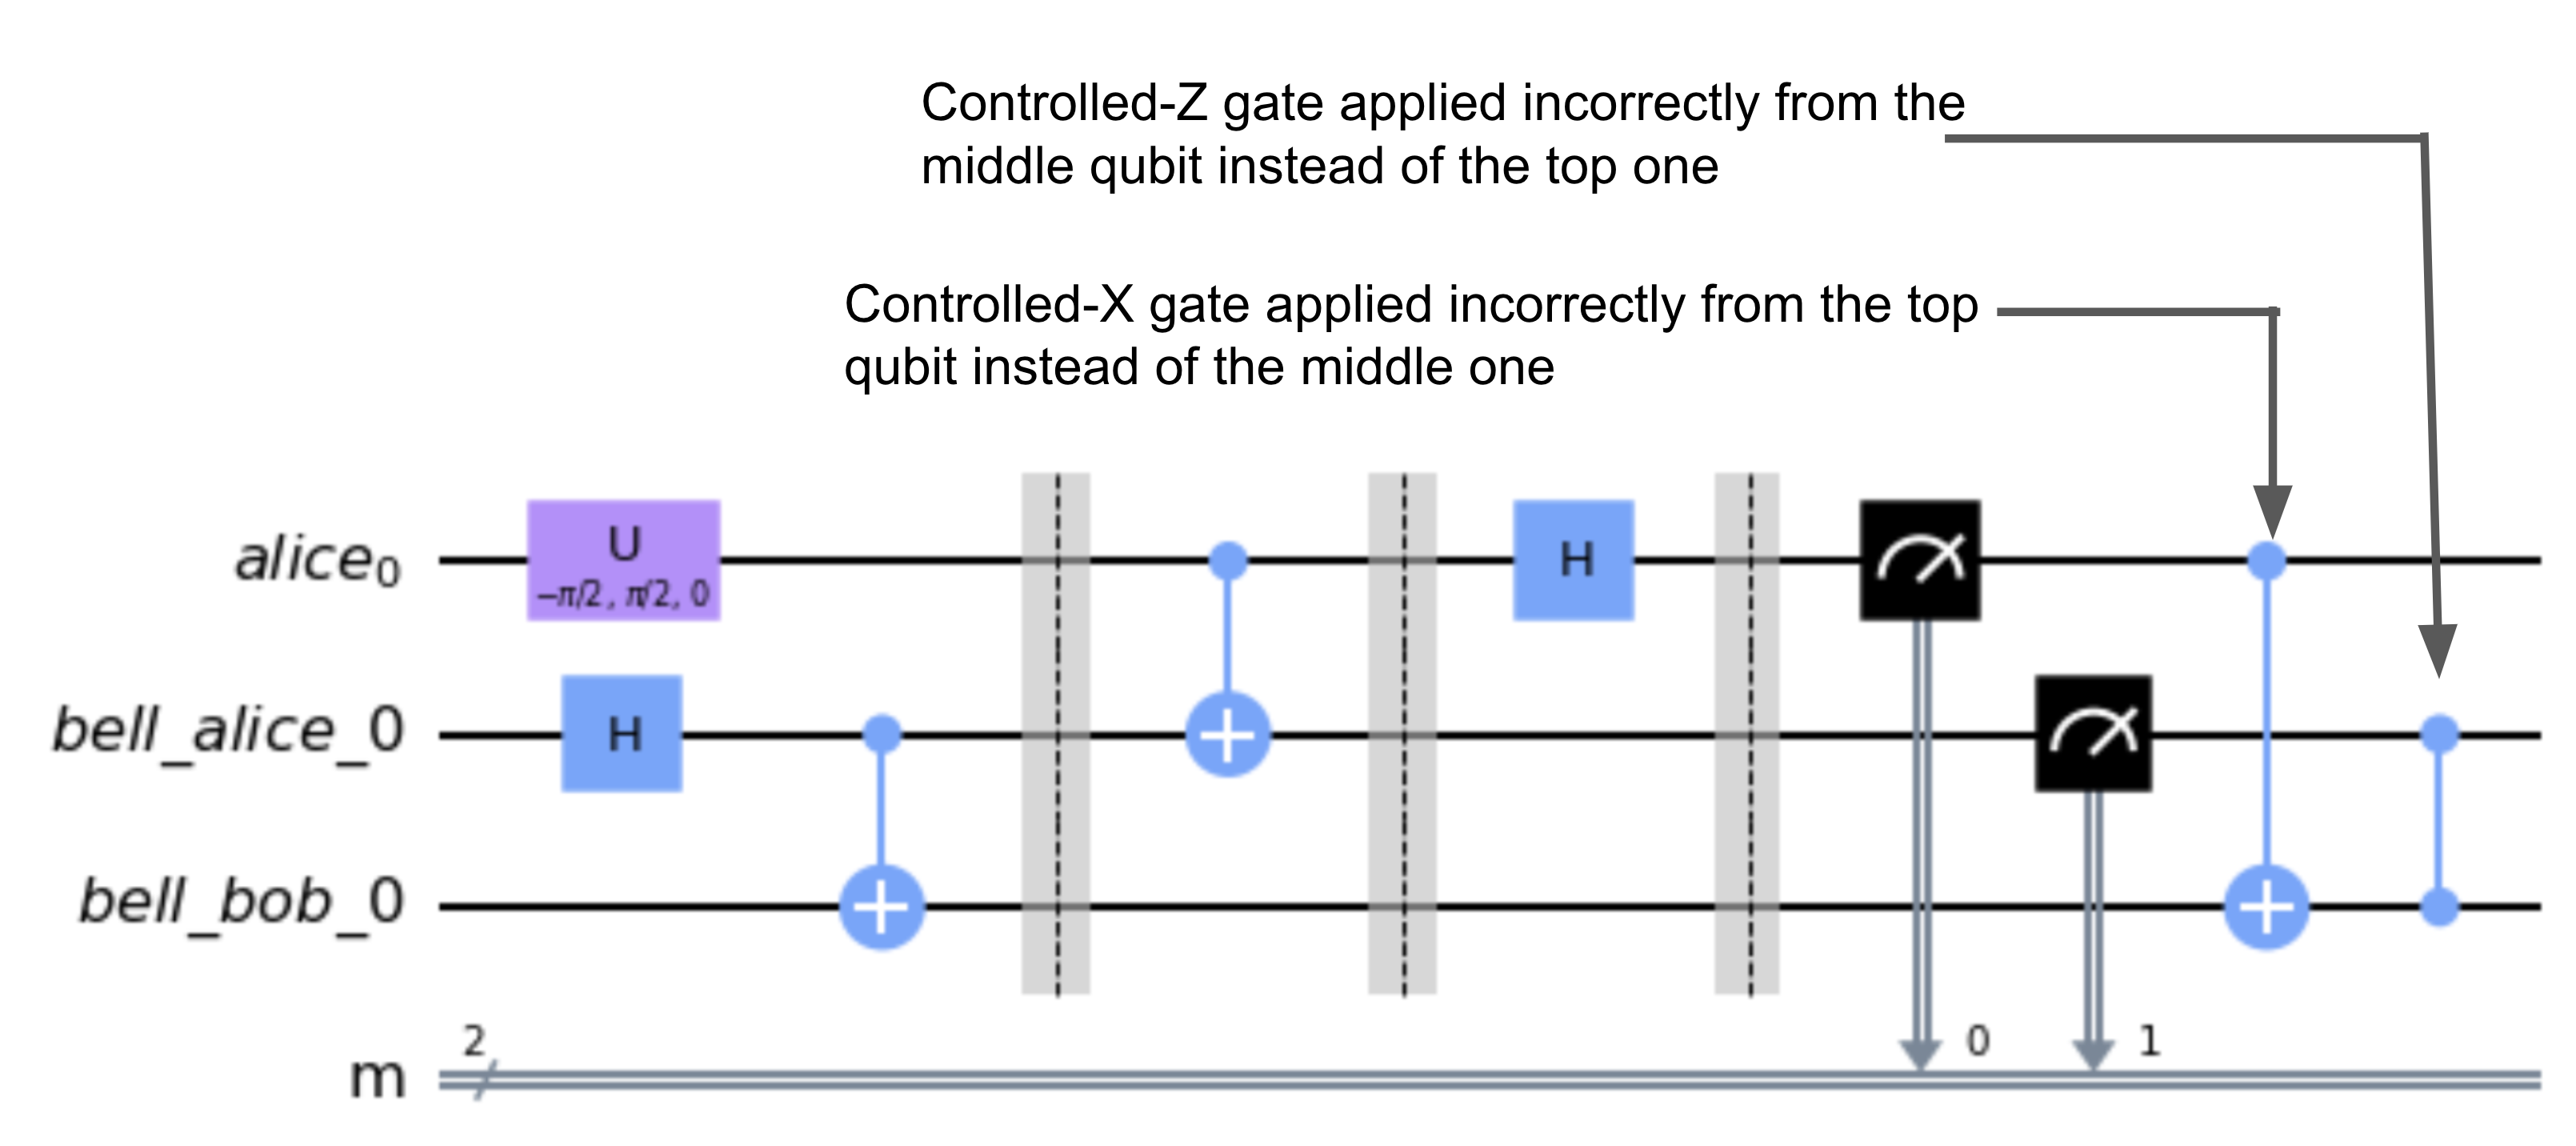
\includegraphics[scale=0.25]{tportwrong.png}

\begin{itemize}
    \item\Points{4}
Complete the table below, \textbf{providing support on the next page}, indicating for which measurements of Alice's qubits, Bob still obtains the correct state on his qubit (\texttt{bell\_bob\_0}).
\begin{center}\Large
\begin{tabular}{ccc}
\multicolumn{2}{c}{Alice's qubit} & Bob obtains the  \\
\texttt{$\mbox{alice}_0$} & \texttt{bell\_alice\_0} & correct state?\\[1em]
0 & 0 & \TF \\[2em]
0 & 1 & \TF \\[2em] 
1 & 0 & \TF \\[2em]
1 & 1 & \TF \\
\end{tabular}
\end{center}
\Continued{}
\item \Points{8} Provide support for your answers here:
\begin{itemize}
    \item \Points{2} Case 00:
    \LeaveSpace{1.5in}
   \item \Points{2} Case 01:
    \LeaveSpace{1.5in}
       \item \Points{2} Case 10:
    \LeaveSpace{1.5in}
       \item \Points{2} Case 11:
    \LeaveSpace{1.5in}
\end{itemize}
\end{itemize}


\clearpage\item\Points{5 extra credit}  If there were a unitary gate $U$ that could conjugate the arbtirary phase~$\phi$ of
a quantum state, then
\[  U\begin{pmatrix*}[r] \cos{\theta} \\ e^{i\phi}\sin{\theta}\end{pmatrix*} = \begin{pmatrix*}[r] \cos{\theta} \\ e^{-i\phi}\sin{\theta}\end{pmatrix*} \]
Arbitrary phase means we do not the value of $\phi$.  Prove that no such
gate $U$ can exist without knowing $\phi$.

\end{enumerate}
\end{assignment}
\Bpage{}

\end{document}
